\documentclass[../../../../main.tex]{subfiles}
\begin{document}

$p$ を $0<p<1$ を満たす実数とする．

\begin{enumerate}
  \item 四面体 $ABCD$ の各辺はそれぞれ確率 $p$ で電流を通すものとする．
  このとき，頂点 $A$ から $B$ に電流が流れる確率を求めよ．
  ただし，各辺が電流を通すか通さないかは独立で，辺以外は電流を通さないものとする．
  \item (1) で考えたような2つの四面体 $ABCD$ と $EFGH$ を図のように頂点 $A$ と $E$ でつないだとき，
  頂点 $B$ から $F$ に電流が流れる確率を求めよ．
\end{enumerate}

\begin{figure}[htbp]
  \centering
  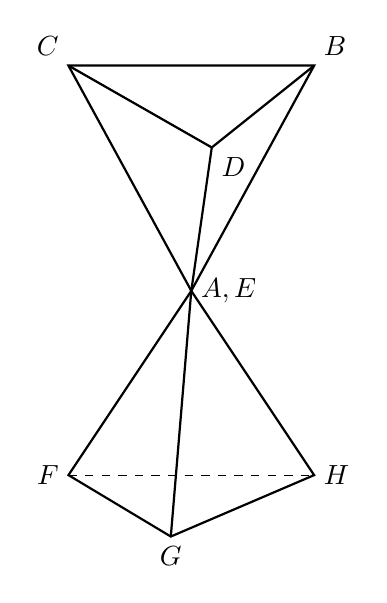
\begin{tikzpicture}[scale=1.3]
    \coordinate (A) at (0,0);

    \coordinate (C) at (-1.2, 2.2);
    \coordinate (B) at (1.2, 2.2);
    \coordinate (D) at (0.2, 1.4);

    \draw[thick] (A) -- (B) -- (C) -- cycle;
    \draw[thick] (A) -- (D);
    \draw[thick] (B) -- (D);
    \draw[thick] (C) -- (D);

    \coordinate (F) at (-1.2, -1.8);
    \coordinate (H) at (1.2, -1.8);
    \coordinate (G) at (-0.2, -2.4);

    \draw[thick] (A) -- (F) -- (G) -- (H) -- cycle;
    \draw[thick] (A) -- (G);
    \draw[dashed] (F) -- (H);

    \node[right] at (A) {$A, E$};
    \node[above right] at (B) {$B$};
    \node[above left] at (C) {$C$};
    \node[below right] at (D) {$D$};
    \node[left] at (F) {$F$};
    \node[below] at (G) {$G$};
    \node[right] at (H) {$H$};
  \end{tikzpicture}
\end{figure}

\end{document}
